\rubrik{årets rebus}

\hfill

Här hittar ni årets rebus. Fundera gärna under kvällen om ni kan lösa den!

\vspace{9pt}

Grattis till Anna och Elsa Ryberg, Elina Ryding, Sofia Damne och Viktor Rehnberg som löste rebusen i vår rebustävling!

\hfill
\begin{figure}[hbt!]
    \centering
    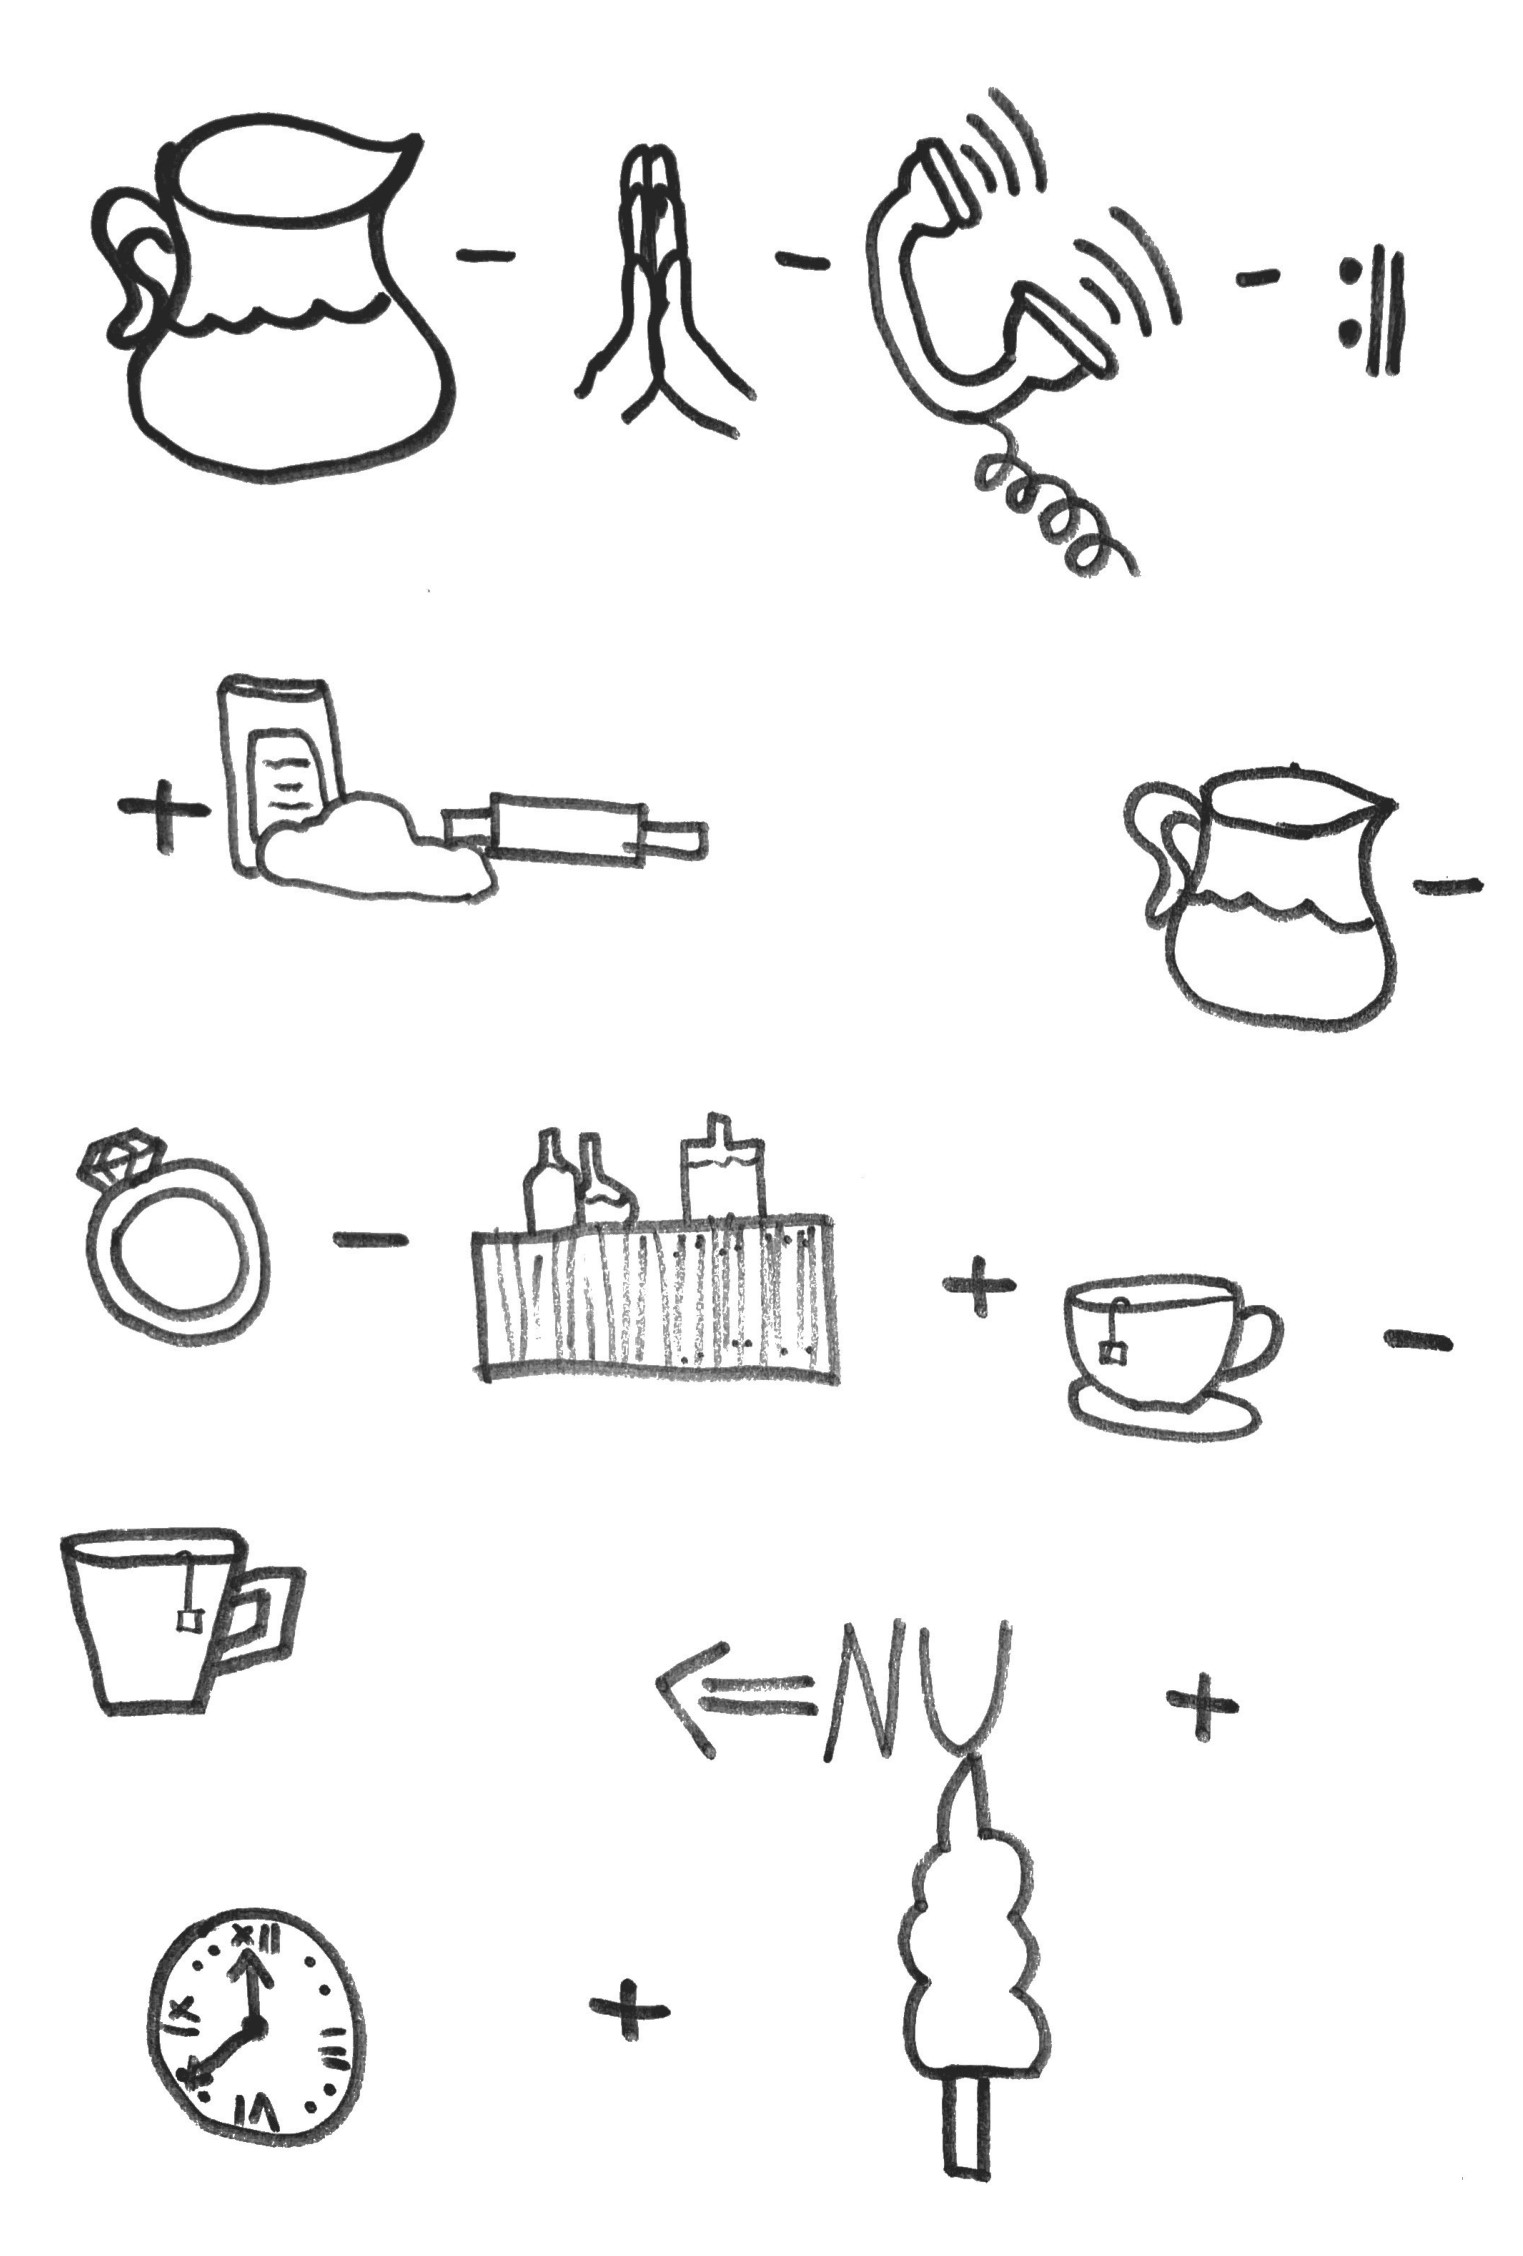
\includegraphics[width=0.5\textwidth]{Bilder/Rebus/Rebus-2022.jpg}
    \label{fig:my_label}
\end{figure}


\vfil

\underrubrik{Lösning på rebus (spoiler!)}

\begin{flushright}

\begin{turn}{180}
och en \textit{en}, alltså \textsc{dåtiden}. Då har vi årets tema: \textsc{Tillbaka till dåtiden}!
\end{turn}

\begin{turn}{180}
Sedan ser vi \textit{nu} med en pil bakåt vilket blir \textit{då}, och så lägger vi till \textit{tid} 
\end{turn}

\begin{turn}{180}
för att sedan lägga till \textit{t(e)} och ta bort \textit{te}. Då har vi fått ordet \textsc{till}.
\end{turn}

\begin{turn}{180}
Efter detta ser vi en ny \textit{tillbringare}. Även där tar vi bort \textit{ring} och \textit{bar} 
\end{turn}

\begin{turn}{180}
 vilket ger \textit{till}. Sedan lägger vi till \textit{baka} och får \textsc{Tillbaka}. 
\end{turn}

\begin{turn}{180} 
Vi ser en \textit{tillbringare} där vi sedan tar bort \textit{be}, \textit{ring} och \textit{re }för repristecknet,
\end{turn}

\end{flushright}
